% Preámbulo
\documentclass[letterpaper]{article}
\usepackage[utf8]{inputenc}
\usepackage[spanish]{babel}

\usepackage{enumitem}
\usepackage{titling}

% Símbolos
	\usepackage{amsmath}
	\usepackage{amssymb}
	\usepackage{amsthm}
	\usepackage{amsfonts}
	\usepackage{mathtools}
	\usepackage{bbm}
	\usepackage[thinc]{esdiff}
	\allowdisplaybreaks

% Márgenes
	\usepackage
	[
		margin = 1.4in
	]
	{geometry}

% Imágenes
	\usepackage{float}
	\usepackage{graphicx}
	\graphicspath{{imagenes/}}
	\usepackage{subcaption}

% Macros
	\newcommand{\sumi}[2]{\sum_{i=#1}^{#2}}
	\newcommand{\dint}[2]{\displaystyle\int_{#1}^{#2}}
	\newcommand{\inte}[2]{\int_{#1}^{#2}}
	\newcommand{\dlim}{\displaystyle\lim}
	\newcommand{\limxinf}{\lim_{x\to\infty}}
	\newcommand{\limninf}{\lim_{n\to\infty}}
	\newcommand{\dlimninf}{\displaystyle\lim_{n\to\infty}}
	\newcommand{\limh}{\lim_{h\to0}}
	\newcommand{\ddx}{\dfrac{d}{dx}}
	\newcommand{\txty}{\text{ y }}
	\newcommand{\txto}{\text{ o }}
	\newcommand{\Txty}{\quad\text{y}\quad}
	\newcommand{\Txto}{\quad\text{o}\quad}
	\newcommand{\si}{\text{si}\quad}

	\newcommand{\etiqueta}{\stepcounter{equation}\tag{\theequation}}
	\newcommand{\tq}{:}
	\renewcommand{\o}{\circ}
	% \newcommand*{\QES}{\hfill\ensuremath{\boxplus}}
	% \newcommand*{\qes}{\hfill\ensuremath{\boxminus}}
	% \newcommand*{\qeshere}{\tag*{$\boxminus$}}
	% \newcommand*{\QESHERE}{\tag*{$\boxplus$}}
	\newcommand*{\QES}{\hfill\ensuremath{\blacksquare}}
	\newcommand*{\qes}{\hfill\ensuremath{\square}}
	\newcommand*{\QESHERE}{\tag*{$\blacksquare$}}
	\newcommand*{\qeshere}{\tag*{$\square$}}
	\newcommand*{\QED}{\hfill\ensuremath{\blacksquare}}
	\newcommand*{\QEDHERE}{\tag*{$\blacksquare$}}
	\newcommand*{\qel}{\hfill\ensuremath{\boxdot}}
	\newcommand*{\qelhere}{\tag*{$\boxdot$}}
	\renewcommand*{\qedhere}{\tag*{$\square$}}

	\newcommand{\suc}[1]{\left(#1_n\right)_{n\in\N}}
	\newcommand{\en}[2]{\binom{#1}{#2}}
	\newcommand{\upsum}[2]{U(#1,#2)}
	\newcommand{\lowsum}[2]{L(#1,#2)}
	\newcommand{\abs}[1]{\left| #1 \right| }
	\newcommand{\bars}[1]{\left \| #1 \right \| }
	\newcommand{\pars}[1]{\left( #1 \right) }
	\newcommand{\bracs}[1]{\left[ #1 \right] }
	\newcommand{\floor}[1]{\left \lfloor #1 \right\rfloor }
	\newcommand{\ceil}[1]{\left \lceil #1 \right\rceil }
	\newcommand{\angles}[1]{\left \langle #1 \right\rangle }
	\newcommand{\set}[1]{\left \{ #1 \right\} }
	\newcommand{\norma}[2]{\left\| #1 \right\|_{#2} }


	\newcommand{\N}{\mathbb{N}}
	\newcommand{\Q}{\mathbb{Q}}
	\newcommand{\R}{\mathbb{R}}
	\newcommand{\Z}{\mathbb{Z}}
	\newcommand{\PP}{\mathbb{P}}
	\newcommand{\1}{\mathbbm{1}}
	\newcommand{\eps}{\varepsilon}
	\newcommand{\ttF}{\mathtt{F}}
	\newcommand{\bfF}{\mathbf{F}}

	\newcommand{\To}{\longrightarrow}
	\newcommand{\mTo}{\longmapsto}
	\newcommand{\ssi}{\Longleftrightarrow}
	\newcommand{\sii}{\Leftrightarrow}
	\newcommand{\then}{\Rightarrow}

	\newcommand{\pTFC}{{\itshape 1er TFC\/}}
    \newcommand{\sTFC}{{\itshape 2do TFC\/}}
    
% Datos
    \title{Gráficas y Combinatoria\\Tarea V}
    \author{Rubén Pérez Palacios\\Profesor: Dr. Octavio Arizmendi Echegaray}
    \date{\today}

% DOCUMENTO
\begin{document}
	\maketitle
    
    \section*{Problemas}

    \begin{enumerate}
		
		\item Sea $G$ una gráfica que contiene un ciclo $C$, y suponga que $G$ contiene un camino de longitud $k$ entre dos vértices de $C$. Muestre que $G$ contiene un ciclo de al menos $\sqrt{k}$ ¿Es esto óptimo?
		
		Consideremos $P$ el número de punto que comparten el cíclo $G$ y el camino de tamaño $k$. Si $\abs{V\pars{P}} >= \sqrt{K}$ entonces $C$ es el cíclo que buscamos. En caso de que $\abs{V\pars{P}} < \sqrt{K}$ por principio de casillas tendra que haber al menos $\sqrt{k}$ puntos concecutivos que no esten en $C$ estos puntos junto con los dos puntos anterior y posterior a ellos forman un ciclo de al menos $\sqrt{k}$ de tamaño.

		\item Muestra que $\Xi_{H\square G} = max(X_H,X_G)$.
		
		\item Sea $G_{n+m}$ la gráfica con $n+m$ vértices que consite en unir un ciclo de tamaño $n$ con un ciclo de tamaño $m$, por un arista.
		
		\begin{enumerate}
			\item Encuentre el número de árboles generadores
			
			Puesto que todo árbol generador tendrá que contener la arista por el cual están unidos los ciclos entonces podemos ver que si los $n$ vértices del ciclo de tamaño $n$ están en un árbol y todos los vértices del ciclo de tamaño $m$ están en un árbol entonces la union de estos arboles junto con la arista generaran un árbol generador de nuestro grafo luego si tomamos un árbol generador de nuestro grafo podemos quitar la arista que une a los ciclos y entonces tendriamos dos arboles cada uno con solo vértices de alguno de los dos ciclos, por lo que hay una biyección entre los arboles generados por los ciclos y los arboles generadores del grafo por lo tanto la respuesta es $n\times m$.

			\item Escribe explicitamente todos los elementos del espacio de ciclos.
			
			La arista que une a los siclos no puede estar en ninguno de los elementos del espacio de cíclo ya que de ser así o alguno de los vertices de esta tendría grado $impar$ o dejaría de ser tener la gráfica solo ciclos como componentes. Ahora por lo que los elementos son

			\[\emptyset, C_n, C_m, C_n+C_m.\]

		\end{enumerate}

		\item ¿Para que parejas $(n,m)$ es $C_n\square C_m$ planar?
		
		Veamos que pasa cuando $n = m = 3$, entonces obtendriamos la siguiente gráfica como proudcto cartesiano

		\begin{figure}[H]
			\centering
			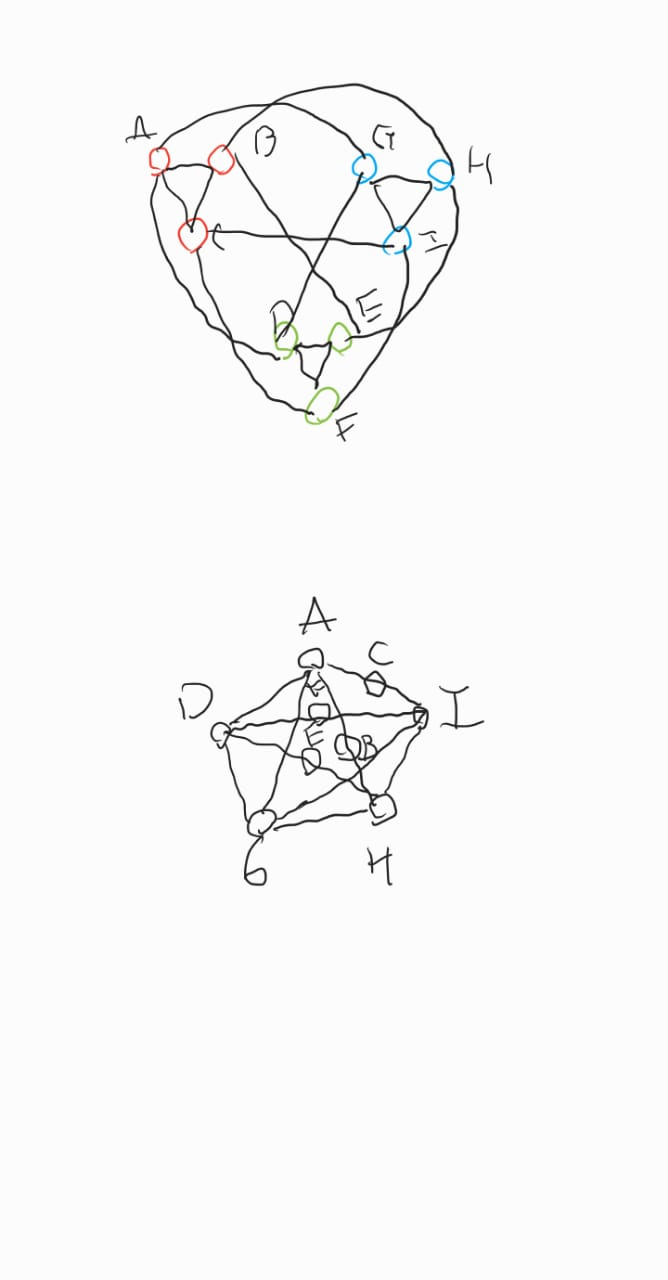
\includegraphics[scale=.25]{1.jpeg}
		\end{figure}
		
		Luego los puntos $3$ generan una subdivisión de $K_5$ por el Teorema de Kuratowski concluimos que $C_3\times C_3$ no es planar.

		Como una subdivisión de $C_3\times C_3$ es una subgrafica de todo $C_n\times C_m$ concluimos que no existen parejas $(n,m)$ tales que $C_n\times C_m$ sea planar.

		\item Para una multigráfica $G = (V,E)$ se define el polinomio de $Tuttle$ por la fórmula
		
		\[T_G(x,y) = \sum_{A\subset E} \pars{x-1}^{k(A) - k(E)} \pars{y-1}^{k(A)+|A|-|V|},\]

		donde $k(A)$ denote el númeor de componentes conexas de la gráfica $(V,A)$.

		Podemos ver que si $E = E_1 + E_2$, $E_1\Cap E_2 = \emptyset$ y $G_i = (V,E_i)$ entonces 
			
		\[T_G = T_{G_1} + T_{G_2}.\]

		También si $E = \emptyset$ entonces
			
		\[T_G = 1.\]

		Esto puesto que

		\[T_G(x,y) = (x-1)^{|V|-|V|}(y-1)^{|V|+0-|V|} = 1.\]
			
		Ahora si $e$ es un puente entonces
			
		\[T_{G} = xT_{G-e},\]

		esto puesto que si $E' = {e}$ con $e$ puente entonces (por la suma directa)

		\[T_G = (x-1)^0(y-1)^0 + (x-1)^1(y-1)^0 = x.\]

		Analogamente si $e$ es un lazo entonces
			
		\[T_{G} = yT_{G-e}.\]

		esto puesto que si $E' = {e}$ con $e$ lazo entonces (por la suma directa)

		\[T_G = (x-1)^0(y-1)^0 + (x-1)^0(y-1)^1 = y.\]

		\begin{enumerate}
			\item Muestra que $T_G=x^iy^j$ si $G$ contiene solo $i$ puentes y $j$ lazos.
			
			Por lo visto anteriormente podemos hacer recursivamente a $T_G$ quitando puentes y lazos y sacando $x$ y $y$ respectivamente y si $E=\emptyset$ entonces $T_G=1$ por lo que 

			\[T_G=x^iy^j.\]
			
			\item Muestra que si $e$ no es un lazo o un puente entonces
			
			\[T_G = T_{G-e} + T_{G/e}.\]

			Esto puesto que

			\begin{align*}
				T_G(x,y) &= \sum_{A\subset E} \pars{x-1}^{k(A) - k(E)} \pars{y-1}^{k(A)+|A|-|V|}\\
				&= \sum_{A\subset E-\set{e}} \pars{x-1}^{k(A) - k(E)} \pars{y-1}^{k(A)+|A|-|V|}\\ &+ \sum_{A\subset E-\set{e}} \pars{x-1}^{k(A\cup\set{e}) - k(E)} \pars{y-1}^{k(A\cup\set{e})+|A\cup\set{e}|-|V|}\\
				&= \sum_{A\subset E-\set{e}} \pars{x-1}^{k(A) - k(E-e)} \pars{y-1}^{k(A)+|A|-|V|}\\ &+ \sum_{A\subset E-\set{e}} \pars{x-1}^{k(A\cup\set{e}) - k(E)} \pars{y-1}^{k(A\cup\set{e})+|A\cup\set{e}|-|V|}\\
				&= T_{G-e} + T_{G/e}
			\end{align*}

			\item Usando $1$ y $2$ demuestra que $T_G(1,1)$ cuenta cuantos árboles generadores tiene $G$.
			
			Esto puesto que si sacamos de manera recursiva todos los puentes y lazos del polinomio por $1$ entonces tendriamos un grafo sin puentes ni lazos (los x, y que sacamos no importan porque se evaluaran en 1), luego como al sacar puentes aseguramos que estos estuvieran en el grafo final...
		\end{enumerate}
    \end{enumerate}

	\end{document}
